\chapter{Architecture Description}
\label{chap:ad}
This chapter provides a summary of the research done for this thesis as an resulting artefact. This artefact takes the form of an architecture description in accordance to ISO42010 and is expressed in terms of the 4+1 view model. The architecture description is also created through following an attribute-driven design approach. Utimately this chapter aims to provide enough specifics, diagrams and details to be useful in future implementations of a multi-tenant system or prototype. 

\section{Adapted Attribute-Driven Design Approach}
 \label{sec:add}
In creating an architecture description, the architect is faced with a range of diverse approaches. Each one of these approaches offers a certain framework for creating the AD and sets certain context and constraints on the design used. One such comprehensive approach to AD design is Attribute-Driven Design (ADD). In its essence, ADD is an approach to defining an AD that uses the software's quality attribute requirements as baseline for the design process \cite{Wojcik2006}. This approach uses an iterative, recursive process to attempt to decompose a system into elements by applying architectural tactics and patterns \cite{Wojcik2006}. The ADD approach provides highly detailed ADs that should satisfy all of the system requirements and quality attributes. This thesis uses a simplified and broad-viewed approach based on ADD in the creation of its architecture description. It does not attempt to completely follow ADD, but instead uses the ADD recommended process as blueprint for creation of the AD.

\section{System Requirements and Constraints}
\label{sec:reqandconstraints}
The following requirements and constraints have been defined after analysis of the use case, literature on multi-tenancy and recommendations of various stakeholders. Table \ref{tab:quality_attributes} outlines the quality attributes that need to be satisfied by our architecture (see Chapter 2, 6, 7). Whereas table \ref{tab:functional_requirements} specifies the core functional requirements for our media marketplace  (see Chapter 4) and table \ref{tab:design_constraints} addresses the constraints placed on our architecture  (see Chapter 4). 


\subsection{Quality Attributes}
\begin{table}[!h]
\centering
\begin{tabularx}{\linewidth}{|l|X|l}
\cline{1-2}
QAR1 & The system shall be scalable under variable tenant loads &   \\
QAR2 & The system shall be highly available in cases of failures &    \\
QAR3 & The system shall be modifiable in terms of adding new tenants &    \\
QAR4 & The system shall be performing highly under variable tenant loads &    \\
QAR5 & The system shall be secure in isolating tenant data &    \\
QAR6 & The system shall be usable in configuring the system to tenant specific requirements &    \\
\cline{1-2}
\end{tabularx}
\caption{Quality Attribute Requirements (QARs) in Priority Order}
\label{tab:quality_attributes}
\end{table}
\newpage

\subsection{Functional Requirements}
\begin{table}[!h]
\centering
\begin{tabularx}{\linewidth}{|l|X|l}
\cline{1-2}
FR1 & The system shall allow the creation of new tenants dynamically with default views &   \\
FR2 & The system shall allow custom views to be deployed per tenant &    \\
FR3 & The system shall allow administrators to add basic configuration info for a tenant &    \\
FR4 & The system shall allow users to create a campaign with specific to and from dates &    \\
FR5 & The system shall allow users to query for available advertising media &    \\
FR6 & The system shall allow users to add selected media to a campaign &    \\
FR7 & The system shall allow users to book campaigns &   \\
FR8 & The system shall allow managers to view booked campaigns and approve or deny them &  \\
FR9 & The system shall allow users to view the status of their booking &   \\
FR10 & The system shall allow media to be searched based on geographic point &   \\
FR11 & The system shall plot available media on a map according to the media's geographic point &   \\
\cline{1-2}
\end{tabularx}
\caption{Functional Requirements (FR) in Priority Order}
\label{tab:functional_requirements}
\end{table}
\newpage

\subsection{Design Constraints}
\begin{table}[!h]
\centering
\begin{tabularx}{\linewidth}{|l|X|l}
\cline{1-2}
DC1 & The system shall be implemented using technologies that are either openly and freely available or provided by the BizSpark program &   \\
DC2 & The system shall be hosted on Windows Azure using either Azure Websites or Azure Web roles combined with either Azure WebJobs or Azure Worker Roles &  \\
DC3 & The system shall be implemented using C\# &    \\
DC4 & The system  shall use the .NET 4.5 framework    \\
DC5 & The system shall use ASP.NET MVC for its front-end &    \\
\cline{1-2}
\end{tabularx}
\caption{Design Constraints (DC) in Priority Order}
\label{tab:design_constraints}
\end{table}

\subsection{Quality Attribute Scenarios}
In accordance to ADD, each Quality Attribute outlined in table \ref{tab:quality_attributes} should be expressed in a stimulus-response form similar to quality attribute scenarios. As such, each QAR has been explicitly broken down from table \ref{table:qar1}, page \pageref{table:qar1} to table \ref{table:qar7} on page \pageref{table:qar7}. These scenarios provides a good stimulus-response breakdown for our quality attributes and allows us to measure the effectiveness of our AD against them. These scenarios are also used in selection of patterns and creation of system elements in the following sections. 

\section{System Elements Decomposition}
After assessing the requirements inputs, quality attribute scenarios and use case further, a broad-overview breakdown of the system has been done into four major container elements. This breakdown outlined in figure \ref{fig:elements}. Each element could be further defined as follow:
\begin{itemize}
\item \textbf{Presentation}: This element is concerned with providing the front-end to our system using ASP.NET MVC and other web technologies. The presentation element should be modifiable by nature allowing it to be altered according to tenant needs and specifications. This element will also include all marketplace related functionality
\item \textbf{Application}: The application element provides background processing and functionality and should be tenant neutral. It is concerned with the back end functionality requirements
\item \textbf{Persistence}: The persistence element is concerned with the storage, retrieval and modification of application data. This includes all service and repository functionality
\item \textbf{Infrastructure}: The infrastructure element contains the components, models and other elements concerned with cross cutting concerns. This element forms part of and is used by all other elements
\end{itemize}

\begin{figure}
\centering
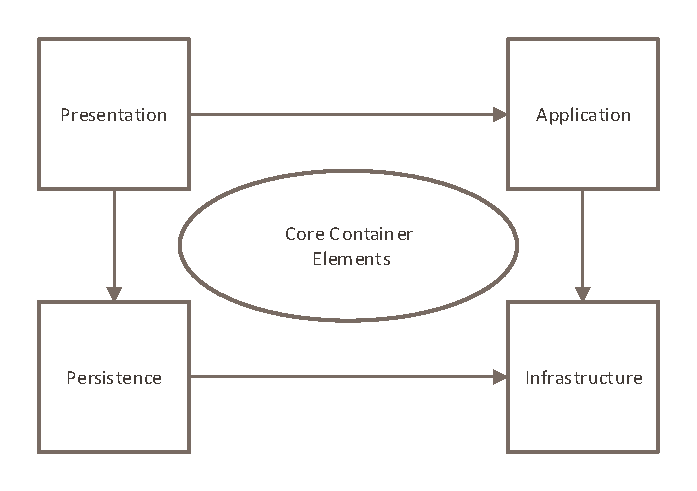
\includegraphics[width=\textwidth]{CoreElements}
\caption{Architecture Core Container Elements}
\label{fig:elements}
\end{figure}


\section{Architectural Drivers}
 \label{sec:arcdrivers}
An analysis of the architectural drivers for each element was made following the techniques outlined by Wood \cite{Wood2007}. This analysis can be seen in appendix \ref{table:architecturaldrivers}. Each requirements is analysed in accordance to its importance and impact or difficulty of implementation. This creates a combination of priorities as outlined by the case study and qualitative interpretation of research conducted. These priorities are then used to select the highest importance, highest impact drivers to architect first. 

\subsection{Candidate Architectural Drivers (CAD)}
Using the architectural drivers and their priorities, all requirements that have a direct influence on the architecture (high and medium impact) have been mapped to each element as shown in figure \ref{fig:designconcernmapping}. This mapping not only allows us to identify the CADs but also indicated three shared requirements amongst all elements nl. QAR1, QAR2 and DC2. These three requirements in effect form three shared concerns that hold a high priority.


\begin{figure}
\centering
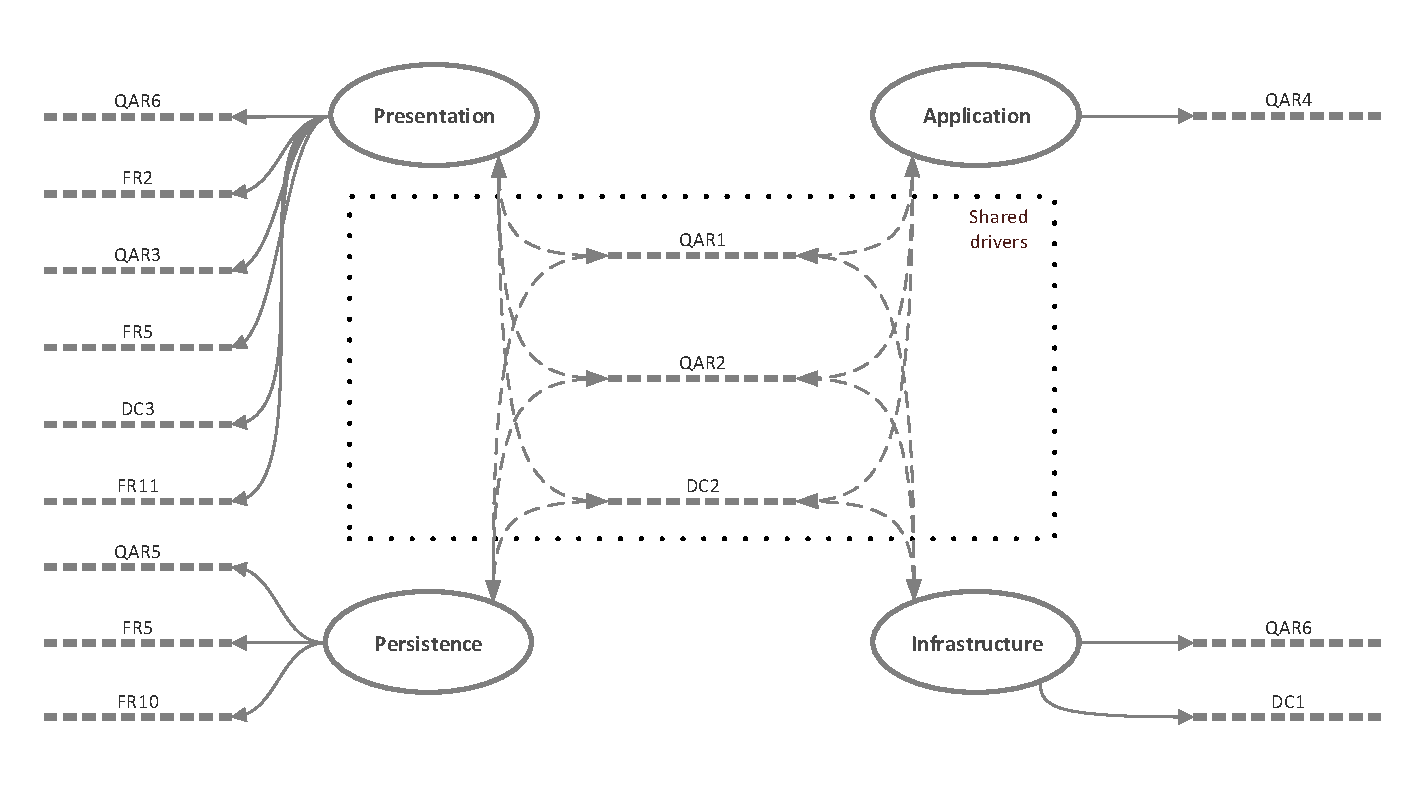
\includegraphics[width=\textwidth]{DesignDriverBreakdown}
\caption{Candidate Architectural Drivers Mapping}
\label{fig:designconcernmapping}
\end{figure}

\section{Design Concerns}
The mapping of candidate architectural drivers seen in figure \ref{fig:designconcernmapping} further allows us to separate requirements that have a direct impact on our architecture from those that do not. After filtering out these requirements, each CAD can be connected to a specific architectural concern as described in Chapter \ref{chapter:architecting} Architecting a Multi-tenant System. By doing this mapping specific requirements are grouped together into specific concerns. Furthermore, these concerns indicate specific problems that needs to be addressed by our AD as well as which requirement can be used to indicate the effectiveness of the solution. The requirement is also used as perspective used in selecting appropriate architectural design patterns to use in the resolution of each concern. See table \ref{table:designconcerns} for the resulting mappings. 


\begin{table}[h]
\centering
\begin{tabularx}{\linewidth}{lXl}
\rowcolor[HTML]{EFEFEF} 
\begin{tabular}[c]{@{}l@{}}Candidat\\ Architectural\\ Driver\end{tabular} & \begin{tabular}[c]{@{}l@{}}Design\\ Concern\end{tabular} & \begin{tabular}[c]{@{}l@{}}Related\\ Sections\end{tabular} \\
QAR1 & Scalability & \ref{sec:scalability} \\
QAR2 & Availability & \ref{sec:availability} \\
QAR6 & Configuration \& Customization & \ref{sec:custandconf} \\
FR2 & Configuration \& Customization & \ref{sec:custandconf} \\
QAR3 & Maintenance & \ref{sec:maintainance} \\
QAR5 & Security & \ref{sec:security} \\
QAR4 & Performance & \ref{sec:performance} \\
DC1 & Technical Constraint & \ref{sec:techconst} \\
DC2 & Technical Constraint & \ref{sec:techconst} \\
\end{tabularx}
\caption{Driver, Concern and Related Section Mappings}
\label{table:designconcerns}
\end{table}

One important aspect to note from the concerns outlined in table \ref{table:designconcerns} is the Environment concern. This specific concern does not require the application of any design patterns as it simply implies some limitations on the technologies that could be used. The following breakdown of technologies have been selected according to this concern (for more information on each of these technologies see appendix \ref{appendix:azure}):
\begin{itemize}
\item \textbf{Web platform}: Azure Cloud Services - Web Role (web server) and Worker Role (background processing)
\item \textbf{Web server}: Internet Information Services (IIS)
\item \textbf{Cache}: Azure Redis Cache
\item \textbf{Persistence}: Azure Document DB, Azure Search, Azure SQL
\item \textbf{Queue}: Azure Storage Queues
\item \textbf{Logging} and Debugging: Elmah, Application Insights
\end{itemize}

\section{Design Concerns and suggested approaches or patterns to addressing them}
In order to address each one of the concerns outlined in table \ref{table:designconcerns} different patterns have been evaluated. The term pattern used in this section refers to the definition by Alexander \cite{Alexander1977-ni}. As a result the term patterns describes any of the following system architecture patterns, design patterns, cloud architecture patterns, workflow patterns and even specific sub-types of patterns of any of the above. In essence, the patterns chosen have been a result of the qualitative interpretation of research done for this paper, personal experience \& skills as well as recommendations from various online sources. In addition the CQRS pattern has been examined specifically for its viability since members of XV have expressed direct interest in implementing it in spite of the domain being only slightly collaborative. 

\subsection{Maintenance Concern}
Implementation of multi-tenancy is the primary principle that is applied to simplify maintenance. Since the current XV platform requires modification of several application instance, uses different code bases for each tenant and has a complex deployment setup, it is clear why this principle will help with this concern. However, implementing multi-tenancy introduces other maintenance issues. In our case, QAR3/4 (see table \ref{tab:qar3}) requires that the system be maintainable in terms of adding new tenants. By using the suggested View Engine solution  discussed in section \ref{sec:viewengine}, we can remove many of the complexities of implementing custom views for tenants. Using a custom view engine will allow us to simply create new views that will be overwrite global ones for each tenant. Although many pure multi-tenant solutions suggest using an approach where all customisation and configuration for tenants is done through configuration, our solution will not allow this. Tenants for our case require extreme degrees of front-end customisation and are provisioned on a monthly basis. This slow provisioning time allows us to use the custom view engine approach instead of using a pure customisation through configuration one. Additionally, the layering pattern has been chosen to help improve maintainability as well. Implementing the layering pattern allows us to decouple our system into different layers or tiers, each responsible for a specific grouping of functions. In contrast to the existing layering pattern implemented in XVA, a layering pattern that utilises the layers suggested by DDD will be used instead. The primary justification for using the DDD layering process is XV's attempt to migrate towards a more domain driven architecture. This decision is also coupled with implementing CQRS.


\subsection{Availability Concern}
No patterns were selected that directly influence our availability concern. Since using Azure already implements various availability assurance mechanisms and their SLA provides terms for high availability this concern has minimal impact on the architecture implementation. However, for the Azure High Availability SLA to apply, we are required to host at least two instances of any of our components. This corresponds to the multiple-instance model suggested for addressing the scalability concern (see section \ref{sec:multiinstance}). Implementation of availability sets should be used to ensure redundancy and remove the impact of planned or unplanned maintenance events as well as failures. Specific application elements will be grouped into an availability set. These availability sets simply assure that our instances that are grouped together are in separate update domains. This means that only one instance of our components will ever be shut down at a time for updates. Azure also automatically deploys application instances to different fault domains. This ensures that hardware failure should affect only one instance of the application and never all of them. 


\subsection{Scalability Concern}

The scalability patterns selected can be found in Appendix A, table \ref{tab:scalability_patterns}.
The patterns mentioned in table \ref{tab:scalability_patterns} are also combined with a multi-instance approach. This means that scalability for our services is achieved by scaling out horizontally by adding more instances. These instances could be of any part of the system. Since a combination of CQRS, QCW and the command pattern is used our presentation layer should be completely independent of executing any commands itself. This has the advantage of being able to scale up the web tier in cases of high query loads. In cases where there is a high command load more instances of the queue handler or application tier can be provisioned. Similarly the query database (if different query and command stores are used) could also be scaled horizontally. Using Azure technologies as required by [DC1/2] allows us to do this scaling on the fly and allows for scaling by metric (see appendix \ref{appendix:azure}). This means that scaling could be setup to be handled automatically and be elastic. This multi-instance approach is also what will primarily be used for addressing our availability concern. These specific patterns were selected due to their relevance as cloud architecture patterns. The CQRS pattern, although criticised as a merely a trending pattern has seen widespread acclaim by various system architects, especially where implemented in combination with DDD. This pattern also directly addresses some of the issues with scaling for multi-tenancy through clean separation of query and command concerns. The QCW pattern is commonly used as supportive pattern to CQRS as it allows an even further degree of separation between the presentation, application and persistence elements. Implementation of this pattern also allows us independent scaling of any of our application elements. The command pattern has been chosen to implement in combination with the other two as it allows delayed execution of commands and helps us to separate the front end from understanding any execution logic. This in effect allows us to move all business, domain logic to the application layer. It also allows us to queue commands to remove concurrency problems. Finally using the auto-scaling pattern has also been considered. The auto-scaling pattern however has not been included in table \ref{tab:scalability_patterns} as it will be used, but not be implemented by our system. This is due to the fact that Windows Azure already implements different auto-scaling strategies that can be implemented purely through configuration in the Azure portal.  



\subsection{Configuration and Customisation Concern}
The External Configuration Store Pattern is used to address the Configuration and Customisation Concern. This pattern simply states that configuration information should be store outside of the application files. Using this approach allows us to centralise configurations for all different instances of our application and its components. Although this pattern refers specifically to application configuration, we will use this pattern to apply to tenant configuration as well. The External Configuration Store pattern suggests the implementation of a management back-end that can be used to manipulate configuration that is separated from the core application.

\section{Security Concern}


\begin{figure}
\centering
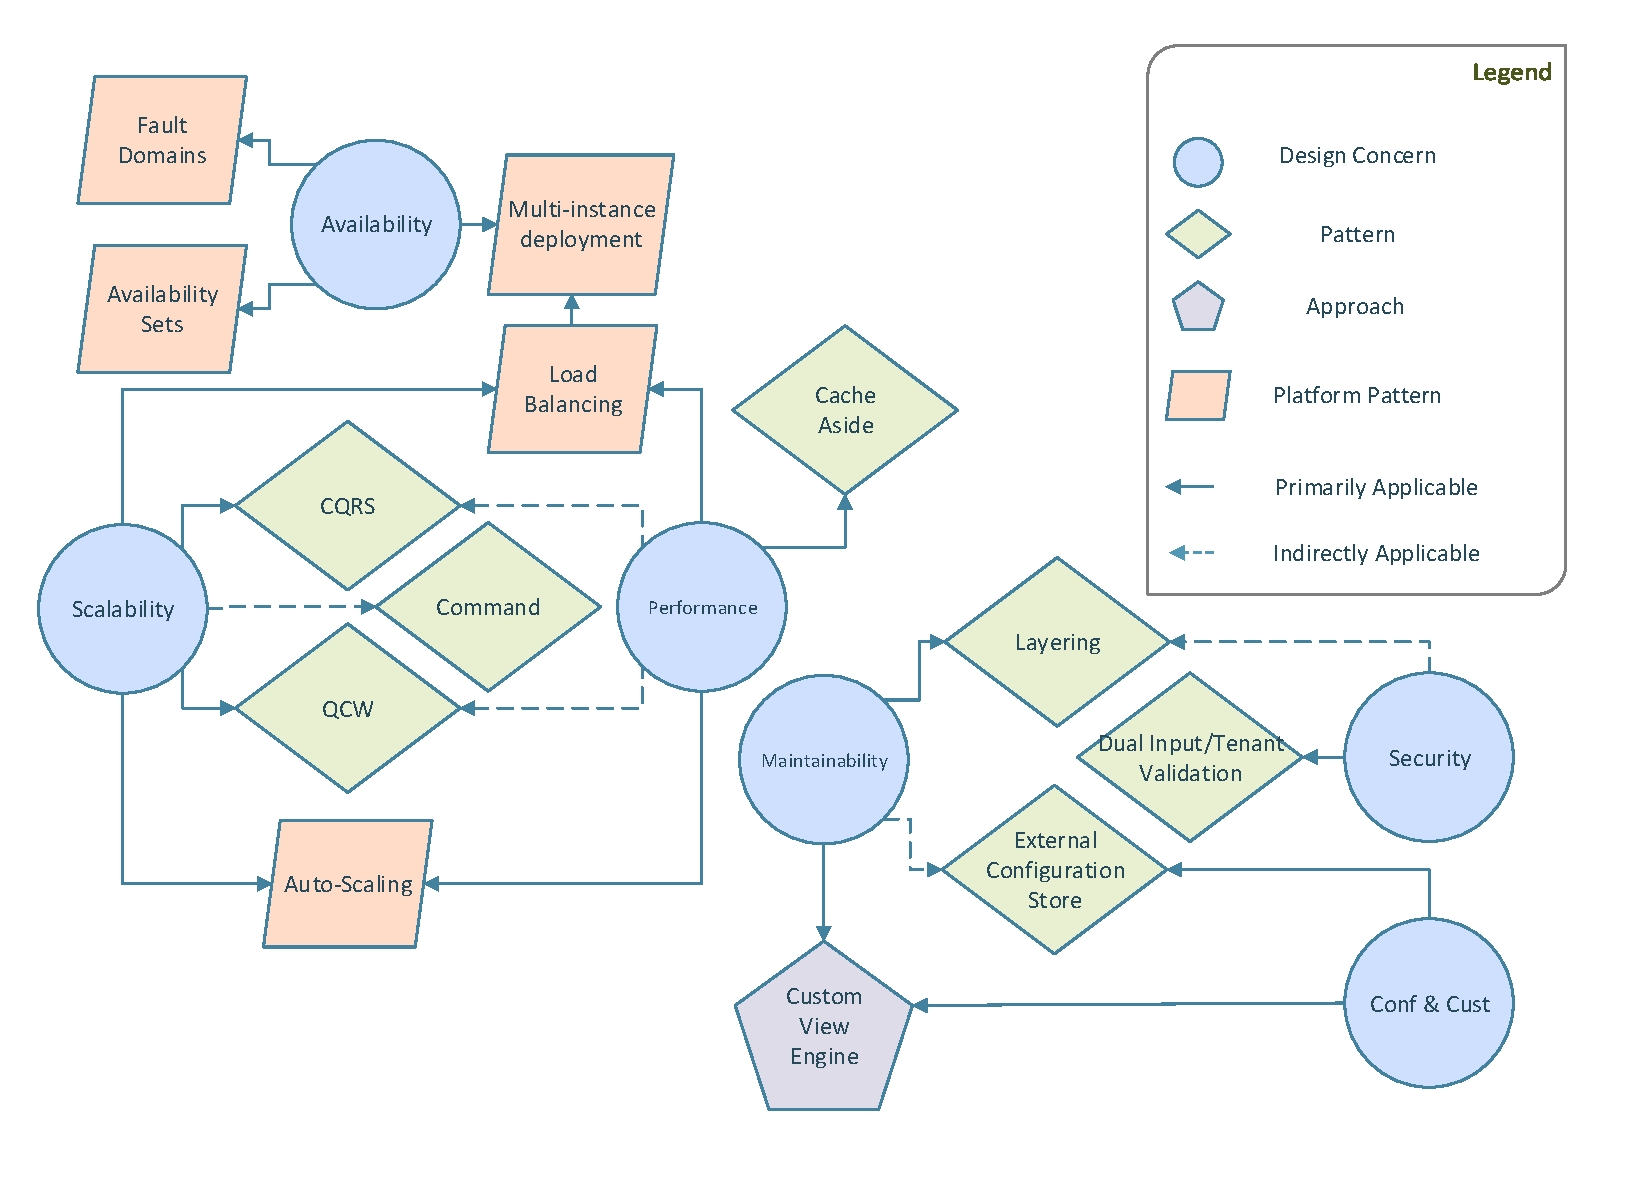
\includegraphics[width=\textwidth]{ConcernPatterns2}
\caption{Design Concerns, Patterns, Approaches and Configurations}
\label{fig:concernpatterns}
\end{figure}
